\documentclass[output=paper, 
colorlinks,
citecolor=brown,
newtxmath
]{langscibook} 
\bibliography{localbibliography}

\author{Rafael Ignacio Zurita\affiliation{Universidad Nacional del Comahue}}
\title{Dispositivos de E/S (periféricos)}  
\abstract{
Además del procesador y memoria, la mayoría de los sistemas embebidos
contienen varios dispositivos de hardware extra. Algunos de estos
dispositivos son específicos a la aplicación, mientras que otros -como los
relojes y puertos seriales- son útiles de una manera general a una gran 
variedad de sistemas distintos.
Los que residen junto con el procesador dentro del mismo chip se los
denomina periféricos internos, u on-chip. Los que se encuentran fuera
del chip donde está el procesador se los denomina de manera opuesta,
es decir, periféricos externos. En este capítulo se detalla la
mayoría de los problemas de software comunes que surgen cuando se programan
periféricos de ambos tipos.

\keywords{sistema embebido, dispositivos de E/S, periféricos, registro de E/S, controladores de E/S, drivers de dispositivos}
}


% add all extra packages you need to load to this file  
\usepackage{tabularx} 

%%%%%%%%%%%%%%%%%%%%%%%%%%%%%%%%%%%%%%%%%%%%%%%%%%%%
%%%                                              %%%
%%%           Examples                           %%%
%%%                                              %%%
%%%%%%%%%%%%%%%%%%%%%%%%%%%%%%%%%%%%%%%%%%%%%%%%%%%% 
%% to add additional information to the right of examples, uncomment the following line
% \usepackage{jambox}
%% if you want the source line of examples to be in italics, uncomment the following line
% \renewcommand{\exfont}{\itshape}
% \usepackage{./langsci/styles/jambox}
\usepackage{./langsci/styles/langsci-lgr}
\usepackage{./langsci/styles/langsci-osl}
\usepackage{langsci-optional}
% \usepackage{langsci-gb4e}
\usepackage{langsci-cgloss}

\usepackage[linguistics]{forest}

\makeatletter
\let\thetitle\@title
\let\theauthor\@author 
\makeatother

\newcommand{\togglepaper}[1][0]{ 
%   \bibliography{../localbibliography}
  \papernote{\scriptsize\normalfont
Esta es una obra derivada oficialmente autorizada por O'Reilly(*) para la materia "Programación de Sistemas Embebidos" de la Facultad de Informática, Universidad Nacional del Comahue. \\ Detalles de la autorización oficial y sus modificaciones al final del capítulo. \\ Libro original: Programming Embedded Systems with C and GNU Development Tools,
Second Edition, by Michael Barr and Anthony Massa. Copyright 2007 O'Reilly Media, Inc., 978-0-596-00983-0
%    \theauthor.
%    \thetitle. 
%    To appear in: 
%    Change Volume Editor \& in localcommands.tex 
%    Change volume title in localcommands.tex
 %   Berlin: Language Science Press. [preliminary page numbering]
  }
 % \pagenumbering{roman}
  \setcounter{chapter}{#1}
  \addtocounter{chapter}{-1}
}


\usepackage[spanish]{babel}
\usepackage[bottom]{footmisc}
\usepackage{tabularx}

\definecolor{aliceblue}{rgb}{0.90, 0.93, 0.96}


\begin{document}

\selectlanguage{spanish}

\chapterfont{\Large\color{LightBlue}} 
\chapter*{Programación de Sistemas Embebidos 2020\\ Makefiles}
{\def\addcontentsline#1#2#3{}\maketitle}
\chapter*{capitulo 3}
{\def\addcontentsline#1#2#3{}\maketitle}
\chapter*{capitulo 4}
{\def\addcontentsline#1#2#3{}\maketitle}
\chapter*{capitulo 5}
{\def\addcontentsline#1#2#3{}\maketitle}

\chapter*{Programación de Sistemas Embebidos 2020\\ Dispositivos de E/S (periféricos)}

\begingroup
\let\clearpage\relax
\cleardoublepage
\hypersetup{linkcolor=blue}
\tableofcontents
\let\clearpage\relax
\cleardoublepage
\endgroup



{\def\addcontentsline#1#2#3{}\maketitle}


\setcounter{page}{1}


\hfill\begin{minipage}{0.8\linewidth} \footnotesize
I consider that the golden rule requires that if I like a program I 
must share it with other people who like it. 
Software sellers want to divide the users and conquer them, making 
each user agree not to share with others. I refuse to break solidarity 
with other users in this way. I cannot in good conscience sign a
nondisclosure agreement or a software license agreement. 
So that I can continue to use computers
without dishonor, I have decided to put together a sufficient body of free software so that I will be able
to get along without any software that is not free.\\
—Richard Stallman 27-sep-1983, Founder of the GNU Project.
\end{minipage}

% \togglepaper[0]

\def\maketitle{

% Titulo 
 \makeatletter
 {\color{bl} \centering \huge \sc \textbf{
\large \vspace*{-8pt} \color{black} Programación de Sistemas Embebidos
 \vspace*{8pt} }\par}
 \makeatother


% Autor
 \makeatletter
 {\centering \small 
 	Departamento de Ingeniería de Computadoras \\
 	Facultad de Informática - Universidad Nacional del Comahue \\
 	\vspace{20pt} }
 \makeatother

}








\section {Registros de estado y de control}

La interfaz entre un procesador embebido y un dispositivo periférico
es un conjunto de registros de estado y control. Estos registros son parte
del hardware del periférico, y sus ubicaciones, sus tamaños (en bits) y el
significado individual de cada bit en cada registro son característicos 
de cada dispositivo. Por ejemplo, 
el significado de los bits de los registros de un dispositivo serial son 
muy diferentes a los
de los contadores o relojes. En esta sección se encuentra explicado la 
manera de manipular el contenido de los registros de estado y control
directamente desde programas en C/C++.

Dependiendo del diseño del procesador y la placa, los dispositivos periféricos
se encuentran localizados en el espacio de memoria del procesador o dentro
del espacio de E/S. De hecho, es común en sistemas embebidos que se incluyan
periféricos de ambos tipos. Se los denomina \textit{periféricos mapeados en memoria}
y \textit{periféricos mapeados en E/S} respectivamente (estos últimos tambien son 
denominados como \textit{aislados}). De los dos tipos, los periféricos
mapeados en memoria son los más fáciles de utilizar y por lo tanto su popularidad
aumenta.

Los registros de estado y control de periféricos mapeados en memoria se pueden
parecer a variables comunes en un programa. Por ejemplo, es posible 
declarar un puntero en C a un registro o bloque de registros, 
y establecer
la dirección explícitamente (valor del puntero). Supongamos el registro
\texttt{puerto\_b} utilizado en el capítulo 2, el cual es mapeado en memoria en la dirección 
física 0x25. La función \texttt{led\_toggle} estudiada en ese capitulo puede ser 
escrita completamente en C, como se muestra a continuación.

\begin{verbatim}
volatile unsigned char * puerto_b = (unsigned char *) 0x25;

void led_toggle(void)
{
    *puerto_b ^= LED_ROJO;    /* Read, xor, and modify. */
}    /* led_toggle() */
\end{verbatim}

Aquí se declara un puntero a un registro de 8 bits y explícitamente se lo
inicializa con  la dirección 0x25. A partir de este momento el puntero al 
registro
trabaja como cualquier puntero a una variable de tipo char de 8 bits.


\subsubsection {Uso de volatile en C o C++}

Note que existe una diferencia muy importante entre 
registros de dispositivos y variables. El contenido de un registro
de dispositivo puede cambiar sin que el programa intervenga o se notifique
del cambio. Esto sucede porque el contenido del registro puede ser modificado
por el hardware del dispositivo. De manera contraria, el contenido de una
variable no cambiará a menos que el programa modifique la misma explícitamente.
Por esa razón, se dice que el contenido de un registro de dispositivo
es volátil, o sujeto a cambiar sin notificación previa.

En C y C++ se debe utilizar la palabra clave volatile cuando se 
declaran punteros a registros de dispositivos.
La misma le indica al compilador que no puede realizar suposiciones acerca
del dato almacenado en esa dirección. Por ejemplo, si el compilador
observa una escritura a una ubicación volátil y luego inmediatamente 
le sigue otra instrucción de escritura a la misma ubicación, el compilador 
no asume  que la primer escritura es innecesaria. En otras palabras, la
palabra clave volatile instruye a la fase de optimización del compilador 
a tratar a esa variable como volátil, y que su conducta no puede ser
predecible en tiempo de compilación.

Prosiguiendo con el ejemplo anterior, se muestra aquí debajo el uso 
de volatile para advertir al compilador acerca del registro \texttt{puerto\_b}:

\begin{verbatim}
volatile unsigned char * puerto_b = (unsigned char *) 0x25;
\end{verbatim}

Es importante notar que es erróneo interpretar, en esta declaración,
que el puntero en si mismo es volátil. De hecho, el valor de la
variable \texttt{puerto\_b} tendrá el valor 0x25 durante toda la ejecución del programa
(a menos que el valor sea modificado por alguna instrucción del programa, por
supuesto). Mas bien es el dato apuntado el que está sujeto a cambiar
sin que el programa intervenga. Este detalle es muy sutil y es fácilmente
confundible al pensar mucho en el tema. Solamente recuerde que la ubicación
de un registro es fija aunque su contenido podría no serlo. Por lo tanto, si se
utiliza la palabra clave volatile, el compilador asumirá lo mismo.

Los otros tipos de registros en dispositivos de E/S (registros en el espacio
de E/S -aislados-) no pueden accederse de la manera anterior, y no
hay una manera estándar de acceder a ellos desde C o C++. 
A estos registros se los accede mediante el uso de instrucciones específicas
de la arquitectura (en lenguaje máquina), las cuales no son soportadas por los 
estándares del lenguaje C o C++. Por lo tanto,
es necesario utilizar rutinas de bibliotecas especiales, o código en lenguaje
ensamblador, usualmente incrustado entre sentencias del programa embebido en C,
para leer y escribir los mismos.


\section {Filosofía del controlador de dispositivo}

\begin{center}
\begin{tabularx}{\textwidth}{|X|}
\hline
\rowcolor{aliceblue}
\textbf{Objetivo de diseño}\\
Al diseñar un controlador de dispositivo (device driver) se debe
tener presente la siguiente meta: ocultar el hardware completamente.\\
\hline
\end{tabularx}
\end{center}

\textit{Un controlador de dispositivo o manejador de dispositivo (en inglés: device driver, o simplemente driver) es el software que controla la operación de un dispositivo de E/S. 
Le permite a la aplicación embebida, o al núcleo del sistema operativo, acceder a 
las funciones del dispositivo, sin que estos tengan que conocer los detalles 
precisos del hardware siendo utilizado, lo que resulta en una abstracción del 
hardware mediante una interfaz de programación.}

Cuando se completó el desarrollo de un sistema embebido, los
módulos controladores de dispositivos (device drivers) deben ser 
las únicas piezas del software en el sistema entero que leen o escriben 
directamente a los registros de estado, control y datos de un periférico. 
En la figura \ref{fig:controladores} se puede observar el diagrama de bloques de alto nivel 
de este concepto.
Existirá un único controlador por cada dispositivo de E/S\footnote{A nivel de 
código fuente, un único controlador puede implicar varios archivos fuentes}.
Además, si un dispositivo genera interrupciones, la rutina de servicio 
de interrupciones que atiende las mismas debe ser parte integral 
del código fuente del controlador de dispositivo de E/S.
En esta sección se explica el por qué se recomienda esta filosofía y cómo
puede ser llevada a cabo.

\begin{figure}
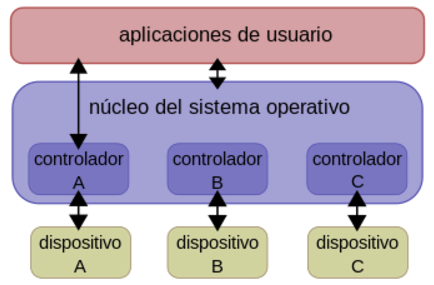
\includegraphics[scale=0.60]{images/controlador.png}
\caption{Diagrama de bloques de un sistema con controladores de dispositivos.}
\label{fig:controladores}
\end{figure}


Por supuesto, intentar ocultar el hardware completamente es difícil. 
Algunas caracterísiticas generales de los dispositivos pueden llegar
a ser visibles siempre, sea cual
sea la interfaz de programación que se diseñe o seleccione.
Esa característica es esperada e inevitable. La meta tiene que ser 
que la interfaz de programación
desarrollada no debería necesitar cambios si el periférico final es reemplazado
con otro de su misma clase general. Por ejemplo, todos los dispositivos de memoria
Flash comparten el concepto de sectores (aunque el tamaño del sector
puede diferir entre chips). Una operación de borrado puede ser realizada
únicamente en un sector entero, y es probable que la aplicación deba indicar
qué sector borrar, o el sistema de archivos. Esa característica del dispositivo 
Flash (sectores) estará visible en la interfaz de programación,
sin poder ser ocultada completamente. De todas maneras, debido a que todas
las memorias de tipo Flash se acceden de a sectores, 
la interfaz desarrollada
para un controlador de memoria Flash debería ser útil con cualquier
dispositivo de memoria similar.

Los controladores de dispositivos para sistemas embebidos son bastante
diferentes a los controladores de dispositivos para estaciones de trabajo (por ej. PC).
En una computadora general, los controladores de dispositivos están
desarrollados con el objetivo de satisfacer los requerimientos del sistema
operativo, debido a que imponen
requerimientos estrictos en la interfaz de software entre el sistema operativo
y controlador de dispositivo. Por ejemplo, el controlador de dispositivo para una placa 
de red particular debe cumplir con la interfaz de software del sistema operativo, 
sin importar las características
y capacidades del hardware subyacente. Los programas de aplicación que 
necesitan utilizar la placa de red están forzados a utilizar la API
de red provista por el sistema operativo, y no tienen acceso directo a la
placa en si misma. En este caso la meta de ocultar el hardware completamente
es alcanzada más fácilmente.

En contraste, el software de aplicación en un sistema embebido  puede acceder al
hardware directamente. De hecho, debido a que todo el software es
vinculado en conjunto en una imagen binaria individual, raramente existe una
distinción entre la aplicación, sistema operativo, y controladores
de dispositivos.
Esta distinción, como así también la aplicación de restricciones de acceso 
al hardware,
son meramente responsabilidades de los desarrolladores de software embebido
(a nivel de código fuente).
Ambas son decisiones de diseño que los desarrolladores deben realizar
concienzudamente. En otras palabras, los programadores de software 
embebido pueden tener más flexibilidad en el diseño del software
que sus pares no embebidos (lo cual no significa que esto sea
una ventaja). De hecho, muchas veces no lo es, y los sistemas embebidos
suelen presentar código fuente pobremente modularizado, y muchas
veces tambien con poco encapsulamiento de los datos de sus módulos.


Los beneficios de un buen diseño del controlador de dispositivo son tres.
Primero, debido a la modularización, la estructura de todo el software
se comprende más fácilmente. Segundo, como hay únicamente un modulo 
que interactúa directamente con los registros de un periférico, el estado
del hardware puede ser verificado mas precisamente. Finalmente, el ultimo 
beneficio pero no por eso menos importante, los cambios en el software que
resultan de los cambios en el hardware están localizados en el controlador
de dispositivo. Todos estos beneficios ayudan a reducir el numero total
de errores en el software embebido.
Pero, se debe estar dispuesto a
realizar el esfuerzo extra que conlleva lograr estos objetivos,
sobre todo en la etapa de diseño de la arquitectura del sistema.

Si acuerda con esta filosofía de ocultar todas las especificaciones del hardware
e interacciones dentro del controlador entonces usualmente debe 
implementar y utilizar los cinco componentes listados a continuación:

\begin{enumerate}
\item Una estructura de datos que se superpone (overlay) a los registros de estado
y control del dispositivo mapeados en memoria
\item Un conjunto de variables para mantener el estado actual del hardware
y del controlador de dispositivo
\item Una rutina para inicializar el hardware a un estado conocido
\item Un conjunto de rutinas que, en su conjunto, presentan una API 
\item Una o varias rutinas de atención de interrupciones

\end{enumerate}

Para realizar una implementación de un controlador de dispositivo lo más simple 
e incremental como sea posible, se debería desarrollar los cinco elementos anteriores
en el orden presentado.

\subsubsection*{Una estructura de datos que se superpone (overlay) a los registros de estado
y control}

El primer paso en el proceso de desarrollo del driver es crear una estructura
(struct), al estilo del lenguaje C, que represente de manera exacta los registros
mapeados en memoria del dispositivo. Generalmente, se necesita estudiar
la hoja de datos del periférico y crear una tabla para los registros
de estado y de control junto con sus desplazamientos (en memoria).
Entonces, comenzando con el registro con la dirección más baja, se 
va completando la tabla de la estructura. Si existen ubicaciones no 
utilizadas o reservadas entre los registros se puede ubicar variables
vacías para ocupar espacio adicional acorde.

Un ejemplo de una estructura de datos del estilo se presenta a continuación.
La misma describe los registros del hardware serial USART presente dentro
del atmega328p. El dispositivo tiene seis registros, dispuestos como se muestra
a continuación en la estructura de datos serial\_st. Cada registro es de 
8 bits y deberían ser manipulados como un unsigned char.

\begin{small}
\begin{verbatim}
struct serial_st
{
    uint8_t data_es;		/* udr0 i/o data */
    uint8_t baud_rate_h;    	/* ubrr0h baud rate high */
    uint8_t baud_rate_l;    	/* ubrr0l baud rate low */;
    uint8_t _reserved;    	/* espacio sin utilizar */
    uint8_t status_control_c;   /* ucsr0c USART Control and Status C */
    uint8_t status_control_b;   /* ucsr0b USART Control and Status B */
    uint8_t status_control_a;   /* ucsr0a USART Control and Status A */
}
\end{verbatim}
\end{small}


Para leer y escribir bits individuales mas fácilmente es una practica común
definir mascaras de bits para usos comunes:

\begin{small}
\begin{verbatim}
#define RECEIVER_ENABLE 0x10        /* RXEN0 Habilitar la recepcion */
#define TRANSMITTER_ENABLE 0x08     /* TXEN0 Habilitar la transmicion */
#define CHARACTER_SIZE_0 0x20       /* UCSZ00 Numero de bits del dato de e/s */
#define CHARACTER_SIZE_1 0x40       /* UCSZ01 Numero de bits del dato de e/s */
#define READY_TO_READ 0x80          /* RXC0 Dato listo para leer */
#define READY_TO_WRITE 0x20         /* UDRE0 Buffer vacio listo para escribir */
\end{verbatim}
\end{small}


\subsubsection*{Un conjunto de variables para mantener el estado actual del hardware
y del controlador de dispositivo}

El segundo paso en el proceso de desarrollo del controlador es definir
qué variables se necesitan para mantener el estado del hardware y 
del controlador de dispositivo. Por ejemplo, en el caso del controlador 
serial probablemente se necesita conocer si el
hardware ha sido inicializado.

Algunos controladores de dispositivos crean tambien \textit{dispositivo de software}.
Esto es un dispositivo puramente lógico, que es implementado en el 
código fuente por encima del controlador del hardware periférico. Por 
ejemplo, es fácil imaginar que más de un reloj por software puede ser 
implementado desde un reloj de hardware (timer/counter). El dispositivo 
de E/S del reloj se configura
para generar un tick de reloj periódico, y el controlador de dispositivo
gestionaría un conjunto de relojes virtuales por software de varias duraciones,
manteniendo información del estado de cada \textit{reloj software}.

\subsubsection*{Una rutina para inicializar el hardware a un estado conocido}

Una vez que se conoce como mantener el estado de los dispositivos 
lógicos y físicos es momento de comenzar a escribir las funciones que 
interactúan y controlan el dispositivo. Es conveniente comenzar 
con la rutina de inicialización del hardware. Además, necesitará
esa rutina primero, y esa es una buena manera de entender como interactuar
con el dispositivo.

\subsubsection*{Un conjunto de rutinas que serán la API para los
usuarios del controlador de dispositivo}

Luego de que se haya inicializado el dispositivo correctamente es
momento de agregar otras funcionalidades al controlador. Es en este
paso en donde se deben establecer los nombres y propósitos de varias 
rutinas, como así también sus respectivos parámetros y valores devueltos.
Una vez definidas es el momento de implementar cada función junto
con un caso de test mínimo. Se presentan ejemplos de tales rutinas
en la siguiente sección.

\subsubsection*{Una o varias rutinas de atención de interrupciones}

Es conveniente diseñar, implementar y verificar la mayoría de las rutinas
del controlador de dispositivo antes de habilitar las interrupciones.
Encontrar el origen de los problemas relacionados con las interrupciones
es muy difícil. Además, si existen errores (bugs) en otros módulos
controladores, la búsqueda del problema relacionado con las interrupciones
puede no tener fin. Por lo que es mejor utilizar 
E/S programada (polling) primero, para obtener el controlador funcionando.
De esta manera se comprenderá cómo trabaja el dispositivo (y que 
realmente esté funcionando) cuando se comienza a buscar la fuente
de los problemas relacionados con las interrupciones. Finalmente, cabe
decir que, desafortunadamente, suele haber casi siempre problemas 
relacionados con las interrupciones cuando se implementa el control por 
software de las mismas.

\section {Controlador de dispositivo serial}

El controlador de dispositivo que se presenta como ejemplo permite
operar un puerto serial. El hardware para este controlador
de dispositivo utiliza un periférico llamado \textit{UART}
(pronunciado 'you-art' y es el acrónimo de
\textit{Universal Asynchronous Receiver Transmitter}) que se encuentra en el atmega328p.
Un UART es un componente de hardware para comunicaciones, que recibe y envía 
información de manera serial y asincrónica. Asincrónico significa que el dato 
que arriba puede llegar en cualquier momento (no está controlado por un reloj), 
similar a la entrada provista por un teclado. 
Un UART acepta un byte de forma paralela desde el procesador, y el dispositivo
lo serializa, transmitiendo cada bit en el momento apropiado. La recepción trabaja
de manera inversa. Los dispositivos UART están disponibles en la mayoría
de las computadoras (embebidas o no), por lo que usualmente se utiliza
para comunicación entre sistemas. Tambien es la interfaz utilizada
por un sin fin de periféricos externos, por lo tanto, implementar un
controlador para dispositivo UART será siempre útil.

Es importante aclarar que el atmega328p tiene en su chip un USART (Universal Synchronous and Asynchronous serial Receiver and Transmitter) que puede trabajar
en modo sincrónico, y también, como periférico SPI maestro. En nuestro
controlador utilizamos únicamente el modo asincrónico no SPI.

Antes de diseñar y desarrollar un controlador de dispositivo 
es importante entender el diagrama de bloques del hardware. Este diagrama
presenta cómo las señales van y vienen desde el periférico al exterior del mismo.

\begin{figure}
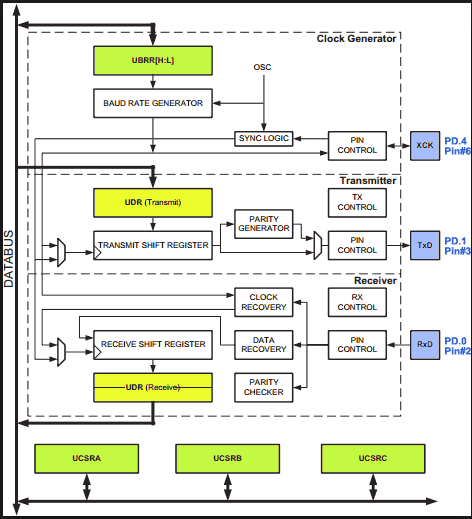
\includegraphics[scale=0.60]{images/usart-block.png}
\caption{Diagrama de bloques del USART en el atmega328p.}
\label{fig:usart-block}
\end{figure}

Típicamente, esta tarea se logra  observando las porciones relevantes de los
esquemáticos, y leyendo las hojas de datos de los diferentes integrados.
Un diagrama de bloques para el puerto serial se muestra en la Figura \ref{fig:usart-block}.
Observe que se han rellenado con colores amarillo y verde los registros
conectados al Databus. Estos son los registros de estado, control y datos que
pueden ser accedidos desde la CPU (conectados al bus). Si existen otros 
registros no conectados al bus con la CPU entonces son registros para uso
interno del hardware del periférico. Los bloques en color celeste son los
componentes que controla el hardware del dispositivo, y se encargan de enviar
señales al exterior (la E/S real).


\subsection*{¿Qué se necesita conocer para controlar el periférico?}
Para este ejemplo de controlador de dispositivo de E/S nos enfocamos únicamente
en el dispositivo USART. La información de sus registros está localizada en la hoja
de datos (en este caso del microcontrolador atmega328p). Mientras se lee esta información
se debe tener en cuenta que la meta es entender varios conceptos, algunos
de ellos son :
\begin{itemize}
\item La estructura de los registros para controlar el periférico, que incluye
el cómo configurar las comunicaciones y como obtener y enviar
datos desde el periférico.
\item Las direcciones de memoria de los registros de estado y de control.
\item El método que se debe utilizar para la operación del periférico (E/S 
programada o con interrupciones).
\item Si se utilizan interrupciones entonces se debe entender bajo qué condiciones
se producen las interrupciones, cómo el controlador de software se informa
de las mismas, y cómo debe atenderlas.
\end{itemize}

\subsection {Registros interfaz}

El primer paso en el disenio de un controlador de dispositivo serial es definir
la interfaz de los registros. En nuestro ejemplo utilizamos
una estructura que se superponga a los registros del USART, los cuales
están mapeados a memoria. La estructura uart\_t se muestra a continuación :


\begin{small}
\begin{verbatim}
typedef struct 
{
    uint8_t data_es;	/* udr0 i/o data */
    uint8_t baud_rate_h;    /* ubrr0h baud rate high */
    uint8_t baud_rate_l;    /* ubrr0l baud rate low */;
    uint8_t _reserved;    /* espacio sin utilizar */
    uint8_t status_control_c;    /* ucsr0c USART Control and Status C */
    uint8_t status_control_b;    /* ucsr0b USART Control and Status B */
    uint8_t status_control_a;    /* ucsr0a USART Control and Status A */
} volatile uart_t
\end{verbatim}
\end{small}

La variable puerto\_serial se utiliza para acceder a los registros
en la dirección 0xc6 (que es la dirección mas baja del registro data\_es),
y es definida así :

\begin{verbatim}
uart_t *puerto_serial = (uart_t *) (0xc6);
\end{verbatim}


\subsection {Variables de estado}

El siguiente paso es definir variables para mantener el estado actual
del hardware. Se declara entonces, en el ejemplo, una estructura
que contiene los parámetros del controlador serial, llamado \texttt{serialparams\_t}.
También, se crea una variable global que contendrá los valores 
de configuración actual definidos en la estructura anterior.

Una variable más, llamada \texttt{initialized} se define, para mantener el estado 
de si el 
controlador de dispositivo está inicializado o no.

\begin{verbatim}
typedef struct
{
    uint8_t dataBits;
    uint8_t stopBits;
    uint8_t baudRate;
    parity_t parity;
} serialparams_t;

serialparams_t serial_params;
\end{verbatim}


\subsection {Rutina de inicialización}

La rutina de inicialización \texttt{serial\_init} configura los parámetros de comunicación
predeterminados.
Los registros del USART son programados utilizando \texttt{serial\_params}, la cual
debe ser inicializada primero.
La variable \texttt{initialized} es utilizada para asegurar que el puerto
serial es configurado únicamente una vez.


\begin{verbatim}
void serial_init()
\end{verbatim}
\footnote{La omisión tiene un propósito, se dejan como tarea para el lector}


\subsection {API del controlador de dispositivo}

Ahora ya es posible incorporar funcionalidad adicional definiendo otras
funciones en el controlador de dispositivo serial.
La API para el controlador de dispositivo serial debería tener, al menos,
funciones para enviar y recibir caracteres. En nuestro ejemplo
se implementan las funciones \texttt{serial\_put\_char} y \texttt{serial\_get\_char}, 
para enviar y recibir caracteres individuales respectivamente.


La función \texttt{serial\_put\_char} debe esperar hasta el que hardware
transmisor del periférico esté listo, y 
luego envía un caracter individual a través del puerto serial (E/S programada).
La transmisión es realizada al escribir el dato al registro de datos del USART.
El siguiente código muestra la función \texttt{serial\_put\_char}.

\begin{verbatim}
void serial_put_char(char c)
\end{verbatim}


La función \texttt{serial\_get\_char} debe esperar hasta que un caracter es recibido, y 
luego es posible leer el mismo desde el registro de datos del puerto serial. 
Para determinar si un caracter ha sido recibido se puede verificar
el bit data ready, del registro de estado del USART. El caracter
recibido es devuelto a la función llamadora. 
El siguiente código implementa esta función.


\begin{verbatim}
char serial_get_char()
\end{verbatim}

Otras funciones extras útiles para anexar a la API del controlador
de dispositivo podrían ser las funciones \texttt{serial\_get\_str()} y \texttt{serial\_put\_str()}
\footnote{API posible: \\ void serial\_put\_str(char * s); \\
char * serial\_get\_str();}.
Debido a que este controlador de dispositivo serial no utiliza interrupciones
el paso final en la filosofía del controlador de dispositivo (implementar
la rutinas que atienden las interrupciones del controlador de dispositivo)
no se implementa.


\subsection *{Verificando (testing) el controlador de dispositivo serial}

Ahora que el controlador de dispositivo está implementado se necesita verificar
que funciona correctamente. Es importante verificar las funciones de la nueva
API de manera individual, 
antes de integrar el controlador junto con el resto del sistema.

Para verificar el controlador debe conectar el puerto serial de la placa
arduino pro mini a la PC. Debido a que los pines del puerto serial de la placa
funcionan con lógica ttl, se debe utilizar un adaptador. Un adaptador
común en estos días es el que adapta estos niveles ttl a USB serial, util 
en caualquier PC.
Luego de conectar el hardware se necesita un programa 'terminal' en la PC, tal
como minicom, picocom, o screen. Ejecute uno de estos programas
y configure el puerto serial del sistema operativo en la PC y la
velocidad de la comunicación, que debe ser la misma que la del driver 
implementado.

La función main demuestra como ejecutar las funcionalidades implementadas
en el controlador de dispositivo.

\begin{small}
\begin{verbatim}
/**********************************************************************
 *
 * Function:    main
 *
 * Description: Exercise the serial device driver.
 * Notes:       
 * Returns:     This routine contains an infinite loop, which can
 *              be exited by entering q.
 *
 **********************************************************************/
int main(void)
{
    char rcv_char = 0;

    /* Configure the UART for the serial driver. */
    serial_init();

    serial_put_char('s');
    serial_put_char('t');
    serial_put_char('a');
    serial_put_char('r');
    serial_put_char('t');
    serial_put_char('\r');
    serial_put_char('\n');

    while (rcv_char != 'q')
    {
        /* Wait for an incoming character. */
        rcv_char = serial_get_char();

        /* Echo the character back along with a carriage return and line feed. */
        serial_put_char(rcv_char);
        serial_put_char('\r');
        serial_put_char('\n');
    }

    /* The embedded program never ends */
    for(;;);

    return 0;
}
\end{verbatim}
\end{small}

Primero, el controlador de dispositivo serial es inicializado llamando 
a \texttt{serial\_init}. Luego, se envían varios caracteres hacia la PC, para 
verificar la función \texttt{serial\_put\_char}. Si el controlador de dispositivo serial
opera correctamente se obtiene el mensaje 'start' en la pantalla terminal
de la PC.

Finalmente un bucle while es ejecutado, chequeando si un caracter
ha sido recibido (llamando a \texttt{serial\_get\_char}). Si se recibe un caracter
en el puerto serial este es enviado nuevamente a la PC a través de un 'eco'.
Si el usuario presiona 'q' en el programa terminal de la PC el programa
embebido finaliza. De otra manera, el bucle continua y comprueba si otro
caracter de entrada arriba volviendo a realizar el 'eco'.


\subsection {Extendiendo la funcionalidad del controlador}


Aunque el controlador es muy básico, tiene funcionalidad como para
escribir una aplicación útil mínima.
Además, el controlador de dispositivo 
presentado es suficiente para aprender acerca de la operación de los UARTs.
La lista a continuación son posibles extensiones que puede realizar
si se desea agregar funcionalidad extra.

\begin{center}
\begin{tabularx}{\textwidth}{|X|}
\hline
\rowcolor{aliceblue}
\textbf{}\\
NOTA: Mantenga esta lista en mente para otros controladores que desarrolle.\\
\hline
\end{tabularx}
\end{center}



\textbf{Configuración seleccionable}

Se puede cambiar \texttt{serial\_init} para que reciba parámetros de entrada,
que permita a la aplicación que utiliza el controlador especificar
los parámetros de comunicación inicial. Por ejemplo, baud rate para
el puerto serial.

\textbf{Verificación de errores}

Es importante para los controladores de hardware realizar un adecuado
chequeo de errores. Se puede comenzar definiendo una lista de códigos
de errores (por ejemplo, errores en los parámetros, errores de hardware, etc)
en la API de controlador.
Las funciones del controlador utilizarían estos códigos para devolver
el estado de la operación si existe un error. De esta manera, la aplicación embebida
utilizando el controlador puede tomar acciones de alto nivel cuando existan
a fallas, y por ejemplo, reintentar la operación.

\textbf{APIs adicionales}

Agregando serial\_get\_str y serial\_put\_str (el cual requiere buffer para
los datos del receptor y transmisor) podría también ser útil. La implementación
de las funciones de tratamiento de cadenas podrían hacer uso de las funciones
serial\_get\_char y serial\_put\_char para implementar el envío individual
de cada elemento.

\textbf{Uso de FIFO}

Algunas veces el hardware de dispositivos UARTs contienen FIFOs (buffers en hardware) 
para los datos recibidos y transmitidos.
Utilizando FIFOs agrega buffer a ambos canales de recepción y transmisión,
logrando que el controlador UART  sea mas robusto. Puede
ser útil incorporar su control por software.

\textbf{Interrupciones}

Activar las interrupciones del UART para la recepción y transmisión es
usualmente mejor que utilizar E/S programada. Por ejemplo, si en la función
\texttt{serial\_get\_char} se utiliza interrupciones se eliminaría la necesidad
de que el controlador deba esperar el caracter entrante. 
La aplicación podría entonces realizar
otras tareas, mientras se espera que el dato sea recibido. 

\section {Consideraciones finales en el diseño de controladores para dispositivos}

La mayoría de los sistemas embebidos tienen mas de un controlador de dispositivo.
De hecho, algunas veces pueden tener muchos. En cuanto
mejore con la experiencia necesita entender la manera en que los
diferentes controladores en el sistema interactúan entre ellos. 
También es importante entender muy bien cómo el software de aplicación 
utiliza los controladores de dispositivos para que pueda diseñar APIs apropiadas.

Con respecto al manejo de errores es necesario primero tener un 
buen entendimiento de todo el diseño
del software, para conocer los posibles problemas que pueden surgir.
Algunas áreas a considerar cuando se realiza el diseño de la arquitectura
del software que incluye varios controladores de software son :

\textbf{Prioridades en las interrupciones}
Si se utilizan interrupciones en los controladores de dispositivos
de un sistema necesita determinar un conjunto apropiado de niveles
de prioridades.


\textbf{Uso de recursos}

Es importante comprender qué recursos son necesarios para cada controlador.
Por ejemplo, imagine el desarrollo de un controlador ethernet para un 
sistema con muy poca memoria.
Es muy probable que esta limitación afecte al esquema de buffer implementado.
El controlador podría manejar el almacenamiento de unos
pocos paquetes entrantes, el cual afectaría al rendimiento de la 
interfaz.

\textbf{Compartir recursos}

Debe tener presente que en ciertas situaciones puede tener múltiple
controladores de dispositivos que necesitan acceder a un hardware común 
(tales como pines de E/S o memoria compartida).
Esto hará difícil localizar errores si el
esquema de divisiones de responsabilidades y uso de recursos
no se piensa a fondo antes.











 
\section{Referencias}

Michael Barr. Programming Embedded Systems in C and C++ 1st Edition. ISBN-13: 978-1565923546
ISBN-10: 1565923545. O'Reilly Media; 1 edition (February 9, 1999)


\section {Licencia y notas de la traducción}

Rafael Ignacio Zurita ({\texttt{rafa@fi.uncoma.edu.ar}) 2016-2020

Este apunte es una traducción del libro de referencia, para
ser utilizado como apunte en la materia de grado
'Programación de Sistemas Embebidos' de la Facultad de Informática,
Universidad Nacional del Comahue.
Se han realizado modificaciones
al contenido para aclarar ciertos detalles o agregar secciones nuevas.
 Tambien se han
modificado todos los archivos fuentes de código, ya que fueron
portados a la plataforma Atmel AVR atmega328.


\begin{center}
\begin{tabularx}{\textwidth}{|X|}
\hline
\rowcolor{aliceblue}
\textit{Esta es una obra derivada del libro de referencia que ha obtenido permiso de O'Reilly para su publicación en PEDCO.}\\
\hline
\end{tabularx}
\end{center}



\subsubsection {Permiso de publicación}

\begin{footnotesize}
\begin{verbatim}
From: Teri Finn <teri@oreilly.com>
Date: Mon, 11 Apr 2016 15:48:58 -0700
Message-ID: <CAOgscZ92-G9iT+=+nnuft4LCoHoe5o8SYPfVEKnS6AKXh8TLyQ@mail.gmail.com>
Subject: Re: Question about permission to translate some parts
To: Rafael Ignacio Zurita <rafa@fi.uncoma.edu.ar>
Content-Type: multipart/alternative; boundary=94eb2c094eeedeba0005303d5a31

--94eb2c094eeedeba0005303d5a31
Content-Type: text/plain; charset=UTF-8

Hi Rafael,

Thank you for providing this further information.  O'Reilly Media is happy
to grant you permission to translation the content you have proposed for
posting to the Moddle site. We're happy you find this information helpful
to the students.

Best regards,

Teri Finn
O'Reilly Media, Inc.

On Thu, Apr 7, 2016 at 10:56 AM, Rafael Ignacio Zurita <
rafa@fi.uncoma.edu.ar> wrote:

[snip]
\end{verbatim}
\end{footnotesize}



%\end{otherlanguage}
% } % foreign language


\end{document}








